\section{Finite Computation}

\subsection{Circuits}

  \begin{definition}
    The most common elementary operations for algorithms are \textbf{logical operators} which can be visualized as a \textbf{gate} in a \textbf{Boolean circuit}. 
  \end{definition}

\subsection{Straight Line Programs}

  \begin{definition}[Straight Line Program]
    A \textbf{straight-line program} is a program that defines certain functions $F, G, H...$ and uses these programs to define variables of the form 
    \begin{align*}
      &\texttt{foo = F(bar,blah)} \\
      &\texttt{foo = G(bar,blah)} \\
      &\texttt{foo = H(bar)} \\
      &\texttt{... = ...}
    \end{align*}
    to come to a result. It is called a straight-line program since it contains no loops or branching (e.g. if/then statements). 

    The \textbf{AON-CIRC programming language} has the AND/OR/NOT operations defined. The binary input variables are of the form 
    \[x = (\texttt{X[0], X[1], ..., X[n-1]})\]
    and output variables of the form 
    \[y = (\texttt{Y[0], Y[1], ..., Y[m-1]})\]
    In every line, the variables on the right-hand side of the assignment operators must either be input variables or variables that have already been assigned a value. We say that an AON-CIRC program $P$ \textit{computes} a function 
    \[f: \{0,1\}^n \longrightarrow \{0,1\}^m\]
    if $P(x) = f(x)$ for every $x \in \{0,1\}^n$.
  \end{definition}

  \begin{example}
    Let the XOR function be defined
    \begin{equation}
      XOR: \{0,1\}^2 \longrightarrow \{0,1\}, \; XOR(a, b) = a + b \pmod{2}
    \end{equation}
    The Boolean circuit for computing $XOR: \{0,1\}^2 \longrightarrow \{0,1\}$ is: 
    \begin{center}
      \begin{circuitikz}[scale=0.3]\draw
        (2,3) node[not port] (not1) {}
        (2,-3) node[not port] (not2) {}
        (12, 3) node[and port] (and1) {}
        (12,-3) node[and port] (and2) {}
        (18,0) node[or port] (or1) {}
        (not1.out) -- (and2.in 1)
        (not2.out) -- (and1.in 2)
        (and1.out) -- (or1.in 1)
        (and2.out) -- (or1.in 2)
        (-4,5.5) node(a) {X[0]}
        (-4,-5.5) node(b) {X[1]}
        (a) -- (not1.in)
        (b) -- (not2.in)
        (a) -- (and1.in 1)
        (b) -- (and2.in 2)
        (21,0) node(y) {Y[0]}
        (or1.out)--(y);
      \end{circuitikz}
    \end{center}
    This can be computed with the straight-line algorithm as such. Given $(a, b)$ as inputs, we have $w_1 = AND(a, b), w_2 = NOT(w_1)$, and $w_3 = OR(a, b)$. Then the algorithm returns $AND(w_2, w_3)$. In Python, this can be programmed: 
    \begin{lstlisting}
      def AND(a, b): return a*b
      def OR(a, b): return 1-(1-a)*(1-b)
      def NOT(a): return 1-a

      def XOR(a, b): 
          w1 = AND(a, b)
          w2 = NOT(w1)
          w3 = OR(a,b)
          return AND(w2, w3)

      print([f"XOR({a},{b})={XOR(a,b)}" for a in [0,1] for b in [0,1]])
      # ['XOR(0,0)=0', 'XOR(0,1)=1', 'XOR(1,0)=1', 'XOR(1,1)=0']
    \end{lstlisting}
  \end{example}

  The way that we've presented the XOR function through Boolean circuits and straight-line programs hints at the following: 

  \begin{theorem}[Equivalence of circuits and straight line programs]
    Let $f: \{0,1\}^n \longrightarrow \{0,1\}^m$ and $s \geq m$ be some number. Then $f$ is computable by a Boolean circuit of $s$ gates if and only if $f$ is computable by an AON-CIRC program of $s$ lines. 
  \end{theorem}

  \begin{definition}
    Let $n, m, s$ be positive integers with $s \geq m$. A \textbf{Boolean circuit} with $n$ inputs, $m$ outputs, and $s$ gates, is a labeled directed acyclic graph (DAG) $G = (V, E)$ with $s+n$ vertices satisfying the following properties: 
    \begin{enumerate}
        \item Exactly $n$ of the vertices have no in-neighbors (i.e. inputs). These vertices known known as \textbf{inputs} and are labeled with the $n$ labels
        \[X[0], X[1], ..., X[n-1]\]
        Each input has at least one out-neighbor. 
        \item The other $s$ vertices are known as \textbf{gates}. Each gate is labeled with $\wedge, \vee$, or $\lnot$. Gates labeled with $\wedge$ (AND) or $\vee$ (OR) have two in-neighbors. Gates labeled with $\lnot$ (NOT) have one in-neighbor. \textbf{Parallel edges} are allowed. 
        \item Exactly $m$ of the gates are also labeled with the $m$ labels 
        \[Y[0], Y[1], ..., Y[m-1]\]
        in addition to their label $\wedge$/$\vee$/$\lnot$. These are known as \textbf{outputs}. 
    \end{enumerate}
    The \textbf{size} of a Boolean circuit is the number of gates it contains. 
  \end{definition}

  Having parallel edges means that an AND or OR gate $u$ can have both its in-neighbors be the same gate $v$. Since $AND(a, a) = OR(a, a) = a$ for every $a \in \{0,1\}$, such parallel gates don't help in computing new values in circuits with AND/OR/NOT gates.

  \begin{center}
    \begin{circuitikz}\draw
      (0, 0) node[and port] (and1) {}
      (5,0) node[and port] (and2) {}
      (and1.out)--(and2.in 1)
      (and1.out)--(and2.in 2)
      ;
    \end{circuitikz}
  \end{center}

  We clarify the definition with the previous example of the function ALLEQ. 

  \begin{figure}[H]
    \centering 
    \begin{circuitikz}[scale=0.4]
      \draw
      (2, 2) node[and port] (and1) {}
      (2, 6) node[not port] (not1) {}
      (2, 10) node[not port] (not2) {}
      (8, 2) node[and port] (and2) {}
      (8, 6) node[and port] (and3) {}
      (8, -2) node[not port] (not3) {}
      (14, 6) node[and port] (and4) {}
      (14, 10) node[and port] (and5) {}
      (14, 14) node[not port] (not4) {}
      (19.5, 12) node[and port] (and6) {}
      (24, 11) node[or port] (or1) {}
      (-4,-1) node(d) {X[3]}
      (-4, 3) node(c) {X[2]}
      (-4, 8) node(b) {X[1]}
      (-4, 12) node(a) {X[0]}
      (a)--(not4.in)
      (a)--(and5.in 1)
      (b)--(not2.in)
      (b)--(and1.in 1)
      (c)--(not1.in) 
      (c)--(and1.in 2)
      (d)--(and2.in 2)
      (d)--(not3.in) 
      (and1.out)--(and2.in 1)
      (not1.out)--(and3.in 2)
      (not2.out)--(and3.in 1)
      (and2.out)--(and5.in 2) 
      (and3.out)--(and4.in 1) 
      (and4.out)--(and6.in 2) 
      (not3.out)--(and4.in 2) 
      (and5.out)--(or1.in 2) 
      (not4.out)--(and6.in 1)
      (and6.out)--(or1.in 1)
      (26, 11) node(y) {Y[0]}
      (or1.out)--(y);
      \draw[color=blue] (-5, -4) rectangle (-3, 16);
      \node[color=blue, above] at (-4, 16) {n Inputs};
      \draw[color=red] (-2, -4) rectangle (25, 16); 
      \node[color=red, above] at (10,16) {s Gates};
      \draw[color=teal] (20.5, 8.5) rectangle (24.5, 13);
      \node[color=teal, below] at (20, 8.5) {m Outputs (Gates)};
      \node at (18, 5) {$s \geq m$};
    \end{circuitikz}
    \caption{} 
    \label{fig:alleq}
  \end{figure}

\subsection{Universal Operations and Gate Sets}

  We have seen that the NAND and AON circuts are can be translated back and forth to each other. Similarly, we can do the same with NAND and AON straight line programs. 

  \begin{definition}[Computability]
    We can also see that a Boolean circuit naturally induces a function defined in the space $\{0,1\}^n$. That is, given Boolean circuit $C$ with $n$ inputs and $m$ outputs, let the \textit{output} of $C$ on the input $x \in \{0,1\}^n$ be denoted $C(x)$. Then, if a function
    \begin{equation}
      f: \{0,1\}^n \longrightarrow \{0,1\}^m
    \end{equation}
    satisfies $f(x) = C(x)$ for all $x \in \{0,1\}^n$, we say that the circuit $C$ \textbf{computes} $f$. 
  \end{definition}

  \begin{definition}[Equivalent in Power]
    Two models are said to be \textbf{equivalent in power} if they can be used to compute the same set of functions. 
  \end{definition}

  Just as we have defined the AON-CIRC program, we can define the notion of computation by a NAND-CIRC program in the natural way. 

  \begin{theorem}[Equivalence Between Circuits and Straight Line Programs]
    AON/NAND circuits and AON/NAND straight-line programs are equivalent in power. Furthermore, for every sufficiently large $s, n, m$ and $f: \{0,1\}^n \longrightarrow \{0,1\}^m$, the following conditions are all equivalent to one another: 
    \begin{enumerate}
      \item $f$ can be computed by a Boolean circuit (with $\wedge, \vee, \lnot$ gates) of at most $O(s)$ gates. 
      \item $f$ can be computed by an AON-CIRC straight-line program of at most $O(s)$ lines
      \item $f$ can be computed by a NAND circuit of at most $O(s)$ gates. 
      \item $f$ can be computed by a NAND-CIRC straight-line program of at most $O(s)$ lines. 
    \end{enumerate}
    By $O(s)$, we mean that the bound is at most $c \cdot s$, where $c$ is a constant that is independent of $n$. For example, if $f$ can be computed by a Boolean circuit of $s$ gates, then it can be computed by a NAND-CIRC program of at most 3$s$ lines, and if $f$ can be computed by a NAND circuit of $s$ gates, then it can be computed by an AON-CIRC program of at most $2s$ lines. 
  \end{theorem}

  We can expand beyond the basis functions of AND/OR/NOT or NAND to a general set of functions 
  \[\mathcal{G} = \{G_0, G_1, ..., G_{k-1}\}\]
  With this, we can define a notion of circuits that use elements of $\mathcal{G}$ as gates and a notion of a \textit{$\mathcal{G}$ programming language} where every line involves assigning to a variable $\texttt{foo}$ the result of applying some $G_i \in \mathcal{G}$ to previously defined or input variables. We state this formally. 

  \begin{definition}[General Straight-line programs]
    Let $\mathcal{F} = \{f_0, f_1, ..., f_{t-1}\}$ be a finite collection of Boolean functions such that
    \[f_i: \{0,1\}^k \longrightarrow \{0,1\}\]
    for some $k_i \in \mathbb{N}$. A \textbf{$\mathcal{F}$ program} is a sequence of lines, each of which assigns to some variable the result of applying some $f_i \in \mathcal{F}$ to $k_i$ other variables. As above, we use $\texttt{X[i]}$ and $\texttt{Y[j]}$ to denote the input and output variables. 

    We say that $\mathcal{F}$ is a \textbf{universal set of operations} (or a \textbf{universal gate set}) if there exists a $\mathcal{F}$ program to compute the function NAND. 
  \end{definition}

  \begin{definition}[Multiplexor]
    
  \end{definition}

  \begin{example}[Multiplexor and Constants are Universal]
    Let $\mathcal{F} = \{IF, ZERO, ONE\}$ where 
    \begin{equation}
      ZERO: \{0,1\} \longrightarrow \{0\}, \;\; ONE: \{0,1\} \longrightarrow \{1\}
    \end{equation}
    are the constant zero and one functions, and 
    \begin{equation}
      IF: \{0,1\}^3 \longrightarrow \{0,1\}, \; IF (a, b, c) = \begin{cases}
        b & a = 1 \\
        c & else 
      \end{cases}
    \end{equation}
    Then, $\mathcal{F}$ is universal since we can use the following formula to compute NAND: 
    \begin{equation}
      NAND(a, b) = IF\big( a, IF(b, ZERO, ONE), ONE\big)
    \end{equation}
  \end{example}

  There are some sets $\mathcal{F}$ that are more restricted in power. For example, it can be shown that if we use only AND or OR gates (without NOT), then we do not get an equivalent model of computation. 

\subsection{Syntactic Sugar}

  Just as we have built the AND, OR, and NOT gates with the NAND gate, we can implement more complex features using our basic building blocks, and then use these new features themselves as building blocks for even more sophisticated features. This is known as \textbf{syntactic sugar}, since we are not modifying the underlying programming model itself, but rather we merely implement new features by syntactically transforming a program that uses such features into one that doesn’t. It makes the language "sweeter" for human use: things can be expressed more clearly, more concisely, or in an alternative style that some may prefer.

  In computer programming, we can define and then execute \textbf{procedures} or \textbf{subroutines}, which are often known as \textit{functions}. 

  \begin{example}[Syntactic Sugar to Define Majority Function]
    We can use syntactic sugar to compute the majority function MAJ as follows, by first defining the procedures NOT, AND, and OR. 
    \begin{lstlisting}
      def MAJ(a,b,c): and1 = AND(a,b)
        and2 = AND(a,c) and3 = AND(b,c)
        or1 = OR(and1,and2) return OR(or1,and3)

      print(MAJ(0,1,1)) # 1
    \end{lstlisting}
  \end{example}

  Note that compared to writing out the full Boolean circuit without any syntactic sugar, one with sugar will can be much simpler. It's the difference between having access to only NAND, or all of NAND, AND, OR, NOT. 

  \begin{definition}
    We call these the programming language NAND-CIRC augmented with the syntax above (for defining procedures) a \textbf{NAND-CIRC-PROC} program. Note that NAND-CIRC-PROC only allows \textit{non-recursive} procedures (that is, procedures that do not take in its return value as its argument). 
  \end{definition}

  We can define conditional (if/then) statements using NAND operators. The idea is to compute the function $IF: \{0,1\}^3 \longrightarrow \{0,1\}$ such that $IF(a, b, c)$ equals $b$ if $a = 1$ and $c$ if $a = 0$. 

  \begin{definition}[Conditional Statement]
    The IF function can be implemented from NANDs as follows: 
    \begin{lstlisting}
      def IF(cond, a, b);
        notcond = NAND(cond, cond) 
        temp = NAND(b, notcond)
        temp1 = NAND(a, cond)
        return NAND(temp, temp1)
    \end{lstlisting}
    The IF function is also known as a multiplexing function, since $cond$ can be thought of as a switch that controls whether the output is connected to $a$ or $b$. 
  \end{definition}
  \begin{proof}
    
  \end{proof}

  \begin{definition}[NAND-CIRC-IF]
    Let NAND-CIRC-IF be the programming language NAND-CIRC augmented with $\texttt{if/then/else}$ statements for allowing code to be conditionally executed based on whether a variable is equal to $0$ or $1$. 
  \end{definition}

  \begin{theorem}
    For every NAND-CIRC-IF program $P$, there exists a standard (i.e. "sugar-free") NAND- CIRC program $P^\prime$ that computes the same function as $P$. 
  \end{theorem}

  We can write the integer addition function as follows: 

  \begin{lstlisting}
    def ADD(A,B):
      Result = [0]*(n+1) 
      Carry = [0]*(n+1) 
      Carry[0] = zero(A[0]) 
      for i in range(n):
        Result[i] = XOR(Carry[i],XOR(A[i],B[i]))
        Carry[i+1] = MAJ(Carry[i],A[i],B[i]) Result[n] = Carry[n]
      return Result
        
    ADD([1,1,1,0,0],[1,0,0,0,0]) # [0, 0, 0, 1, 0, 0]
  \end{lstlisting}

  where $\texttt{zero}$ is the zero function, and $\texttt{MAJ, XOR}$ correspond to the majority and XOR functions respectively. Note that in here, $n$ is a \textit{fixed integer} and so for every such $n$, $\texttt{ADD}$ is a \textit{finite} function that takes as input $2n$ bits and outputs $n+1$ bits. Note that the $\texttt{for}$ loop isn't anything fancy at all; it is just shorthand notation of simply repeating the code $n$ times. By expanding out all the features, for every value of $n$ we can translate the above program into a standard ("sugar-free") NAND-CIRC program. Note that the sugar free NAND-CIRC program to adding two-digit binary numbers consists of 43 lines of code, with a Boolean circuit of 15 layers. 

  We can in fact prove the following theorem that gives an upper bound on the addition algorithm. 

  \begin{theorem}[Addition using NAND-CIRC programs]
    For every $n \in \mathbb{N}$, let 
    \begin{equation}
      ADD_n : \{0,1\}^{2n} \longrightarrow \{0,1\}^{n+1}
    \end{equation}
    be the function that, given $x, x^\prime \in \{0,1\}^n$, computes the representation of the sum of the numbers that $x$ and $x^\prime$ represent. Then, for every $n$ there is a NAND-CIRC program to compute $ADD_n$ with at most $9n$ lines. 
  \end{theorem}

  Once we have addition, we can use grade-school algorithm of multiplication to obtain multiplication as well. 

  \begin{theorem}[Muliplication using NAND-CIRC programs]
    For every $n$, let 
    \begin{equation}
      MULT_n : \{0,1\}^{2n} \longrightarrow \{0,1\}^{2n}
    \end{equation}
    be the function that, given $x, x^\prime \in \{0,1\}^n$, computes the representation of the product of the numbers that $x$ and $x^\prime$ represent. Then, there is a constant $c$ such that for every $n$, there is a NAND-CIRC program of at most $cn^2$ that computes the function $MULT_n$.\footnote{As we have seen in DSA, \textit{Karatsuba's algorithm} allows us to actually compute that there is a NAND-CIRC program of $O(n^{\log_2 3})$ lines to compute $MULT_n$. }
  \end{theorem}

  The LOOKUP function tells us the value of a certain entry. 

  \begin{definition}[Lookup function]
    For every $k$, the \textbf{lookup function} of order $k$, 
    \[LOOKUP_k: \{0,1\}^{2^k} \times \{0,1\}^k \simeq \{0,1\}^{2^k + k} \longrightarrow \{0,1\}\]
    (where $\simeq$ denotes isomorphism) is defined as follows: For every $x \in \{0,1\}^{2^k}$ and $i \in \{0,1\}^k$, 
    \[LOOKUP_k (x, i) = x_i\]
    where $x_i$ denotes the $i$th entry of $x$ in binary representation. 
  \end{definition}

  \begin{theorem}
    For every $k > 0$, there is a NAND-CIRC program that computes the function $LOOKUP_k: \{0,1\}^{2^k + k} \longrightarrow \{0,1\}$. The number of lines in this program is at most $4 \cdot 2^k$. This also means that $LOOKUP_k$ can be computed by a Boolean circuit (with AND, OR, and NOT) gates of at most $8 \cdot 2^k$ gates. 
  \end{theorem}

\subsection{Computability of Finite Functions}

  In fact, we can compute \textit{every} finite function with a large enough Boolean (or equivalently, NAND) circuit. 

  \begin{theorem}[Universality of Finite Functions]
    There exists some constant $c > 0$ such that for every $n, m > 0$ and function
    \[f: \{0,1\}^n \longrightarrow \{0,1\}^m\]
    there is a NAND-CIRC program/NAND circuit,  with at most $c \cdot m 2^n$ lines/gates that computes the function $f$. 
  \end{theorem}

  Since the models of NAND circuits, NAND-CIRC programs, and AON-CIRC programs, and Boolean circuits are all equivalent to one another, we can restate the theorem as such. 

  This may not be so surprising actually. After all, a finite function $f: \{0,1\}^n \longrightarrow \{0,1\}^m$ can be represented by simply the list of its outputs for each one of the $2^n$ input values. So it makes sense that we could write a NAND-CIRC program of similar size to compute it. 

  \begin{definition}
    For every $n, m \in \{1, 2, ..., 2s\}$, let $SIZE_{n, m} (s)$ denote the set of all functions $f: \{0,1\}^n \longrightarrow \{0,1\}^m$ such that $f \in SIZE(s)$. We denote $SIZE_n (s)$ to be just $SIZE_{n,1} (s)$. For every integer $s \geq 1$, we let 
    \[SIZE(s) = \bigcup_{n, m \leq 2s} SIZE_{n, m} (s)\]
    be the set of all functions $f$ that can be computed by NAND circuits of at most $s$ gates (or equivalently, by NAND-CIRC programs of at most $s$ lines). 
  \end{definition}

  We can summarize the equivalence of these models below: 
  \begin{center}
    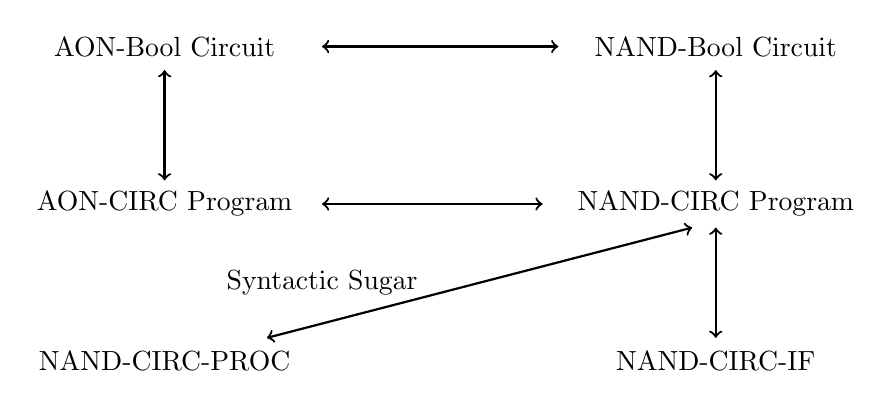
\begin{tikzpicture}
      \node at (0, 0) {AON-Bool Circuit};
      \node at (0, -2) {AON-CIRC Program};
      \node at (7, 0) {NAND-Bool Circuit};
      \node at (7, -2) {NAND-CIRC Program};
      \node at (0, -4) {NAND-CIRC-PROC};
      \node at (7, -4) {NAND-CIRC-IF};
      \draw[<->, thick] (0, -0.3)--(0, -1.7);
      \draw[<->, thick] (7, -0.3)--(7, -1.7);
      \draw[<->, thick] (7, -2.3)--(7, -3.7);
      \draw[<->, thick] (2, 0)--(5,0);
      \draw[<->, thick] (2, -2)--(4.8,-2);
      \draw[<->, thick] (6.7, -2.3)--(1.3, -3.7);
      \node at (2, -3) {Syntactic Sugar};
    \end{tikzpicture}
  \end{center}

\section{Code as Data, Data as Code}

  A program is simply a sequence of symbols, each of which can be encoded in binary using (for example) the ASCII standard. Therefore, we can represent every NAND-CIRC program (and hence also every Boolean circuit) as a binary string. This means that we can treat circuits or NAND-CIRC programs both as instructions to carrying computation and also as \textit{data} that could potentially be used as \textit{inputs} to other computations. That is, \textbf{a program is a piece of text, and so it can be fed as input to other programs}. 

\subsection{Representing Programs as Strings}

  We can represent programs or circuits as strings in many ways. For example, since Boolean circuits are labeled directed acyclic graphs, we can use the \textit{adjacency matrix} representations. A simpler way is to just interpret the program as a sequence of letters and symbols. For example, the NAND-CIRC program $P$: 
  \begin{lstlisting}
  temp_0 = NAND(X[0],X[1])
  temp_1 = NAND(X[0],temp_0)
  temp_2 = NAND(X[1],temp_0)
  Y[0] = NAND(temp_1,temp_2)
  \end{lstlisting}
  is simply a string of 107 symbols which include lower and upper case letters, digits, the underscore character, equality signs, punctuation marks, space, and the "new line" markers, all of which can be encoded in ASCII. Since every symbol can be encoded as a string of $7$ bits using the ASCII encoding, the program $P$ can be encoded as a string of length $7 \cdot 107 = 749$ bits. Therefore, we can prove that \textit{every} NAND-CIRC program can be represented as a string in $\{0,1\}^*$. 

  Furthermore, since the names of the working variables of a NAND-CIRC program do not affect its functionality, we can always transform a program to have the form of $P^\prime$, where all variables apart from the inputs and outputs, have the form $\texttt{temp}_0$, $\texttt{temp}_1$, ... Moreover, if the program has $s$, lines, then we will never need to use an index larger than $3s$ (since each line involves at most three variables), and similarly, the indices of the input and output variables will all be at most $3s$. Since a number between $0$ and $3s$ can be expressed using at most $\left\lceil{\log_{10} (3s+1)} \right\rceil = O(\log s)$ digits, each line in the program (which has the form $\texttt{foo = NAND(bar, blah)}$), can be represented using $O(1) + O(\log s) = O(\log s)$ symbols, each of which can be represented by $7$ bits. This results in the following theorem 

  \begin{theorem}[Representing programs as strings]
  There is a constant $c$ such that for $f \in SIZE(s)$, there exists a program $P$ computing $f$ whose string representation has length at most $cs \log s$. 
  \end{theorem}

\subsection{Counting Programs}

  We can actually see that the number of programs of certain length is bounded by the number of strings that represent them. 

  \begin{theorem}[Counting programs]
  For every $s \in \mathbb{N}$, 
  \[|SIZE(s)| \leq 2^{O(s \log s)}\]
  That is, there are at most $2^{O (s \log s)}$ functions computed by NAND-CIRC programs of at most $s$ lines. This gives a limitation on NAND-CIRC programs running on at most a given number of $s$ lines. 
  \end{theorem}

  Note that a function mapping $\{0,1\}^2 \longrightarrow \{0, 1\}$ can be identified with a table of its four values on the inputs 00, 01, 10, 11. A function mapping $\{0,1\}^3 \longrightarrow \{0,1\}$ can be identified with the table of its 8 values on the inputs 000, 001, 010, 011, 100, 101, 110, 111. More generally, every function 
  \[F: \{0,1\}^n \longrightarrow \{0,1\}\]
  is equal to the number of such tables which is $2^{2^n}$. Note that this is a \textit{double exponential} in $n$, and hence even form small values of $n$ (e.g. $n = 10$), the number of functions from $\{0,1\}^n \longrightarrow \{0,1\}$ is large. 

  \begin{theorem}[Counting argument lower bound]
  The shortest NAND-CIRC program to compute $f: \{0,1\}^n \longrightarrow \{0,1\}$ requires more than $\delta \cdot 2^n / n$ lines. That is, there exists a constant $\delta > 0$ such that for every sufficiently large $n$, there exists $f: \{0,1\}^n \longrightarrow \{0,1\}$ such that $f \not\in SIZE\Big( \frac{\delta 2^n}{n}\Big)$. The constant $\delta$ can be proven to be arbitrarily close to $\frac{1}{2}$. 
  \end{theorem}

  We already know that every function mapping $\{0,1\}^n$ to $\{0,1\}$ can be computed by an $O(2^n / n)$ line program. The previous theorem shows that some functions do require an astronomical number of lines to compute. That is, \textbf{some functions $f: \{0,1\}^n \longrightarrow \{0,1\}$ cannot be computed by a Boolean circuit using fewer than exponential (in $n$) number of gates}. 

\subsection{Tuples Representation}

  ASCII is a fine representation of programs, but we can do better. That is, give a NAND-CIRC program with lines of the form 
  \begin{lstlisting}
  blah = NAND(baz, boo)
  \end{lstlisting}
  We can encode each line as the triple $\texttt{(blah, baz, boo)}$. Furthermore, we can associate each variable with a number and encode the line with the 3-tuple $(i, j, k)$. Expanding on this, we can associate every variable with a number in the set
  \[[t] = \{0, 1, 2, ..., t-1\}\]
  where the first $n$ numbers $\{0, ..., n-1\}$ correspond to input variable, the last $m$ numbers $\{t-m, ..., t-1\}$ correspond to the output variables, and the intermediate numbers $\{n, ..., t-m-1\}$ correspond to the remaining variables. 

  \begin{definition}[List of tuples representation]
  Let $P$ be a NAND-CIRC program of $n$ inputs, $m$ outputs, and $s$ lines, and let $t$ be the number of distinct variables used by $P$. The \textbf{list of tuples representation of $P$} is the triple $(n, m, L)$, where $L$ is the list of triples of the form $(i, j, k)$ for $i, j, k \in [t]$. We assign a number for a variable of $P$ as follows:
  \begin{enumerate}
      \item For every $i \in [n]$, the variable $\texttt{X[i]}$ is assigned to the number $i$. 
      \item For every $j \in [m]$, the variable $\texttt{Y[j]}$ is assigned to the number $t - m + j$.
      \item Every other variable is assigned a number in $\{n, n+1, ..., t-m-1\}$ in the order in which the variable appears in the program $P$. 
  \end{enumerate}
  This is usually the default representation for NAND-CIRC programs, so we will call it "the representation" shorthand. The program could be represented as the list $L$ instead of the triple $(n, m, L)$. 
  \end{definition}

  \begin{example}
  To represent the XOR program of lines 
  \begin{lstlisting}
  u = NAND(X[0], X[1])
  v = NAND(X[0], u) 
  w = NAND(X[1], u)
  Y[0] = NAND(v, w)
  \end{lstlisting}
  we represent it as the tuple 
  \[L = \big( (2, 0, 1), (3, 0, 2), (4, 1, 2), (5, 3, 4)\big) \]
  Note that the variables $\texttt{X[0], X[1]}$ are given the indices $0, 1$, the variable $\texttt{Y[0]}$ is given the index $5$, and the variables $\texttt{u, v, w}$ are given the indices $2, 3, 4$. 
  \end{example}

  So, if $P$ is a program of size $s$, then the number $t$ of variables is at most $3s$. Therefore, we can encode every variable index in $[t]$ as a string of length $l = \left\lceil{\log(3s)}\right\rceil$ (in binary), by adding leading zeros as needed. Since this is fixed-length encoding, it is prefix free, and so we can encode the list $L$ of $s$ triples as simply as the string of length $3ls$ obtained by concatenating all of these encodings. 

  Letting $S(s)$ be the length of the string representing the list $L$ corresponding to a size $s$ program, we get
  \[S(s) = 3sl = 3s \left\lceil{\log(3s)}\right\rceil\]

\subsection{NAND-CIRC Interpreter in NAND-CIRC}

  Since we can represent programs as strings, we can also think of a program as an input to a function. In particular, for every natural number $s, n, m > 0$, we define the function
  \[EVAL_{s, n, m} : \{0,1\}^{S(s) + n} \longrightarrow \{0,1\}^m\]
  as such: Given that $px$ is the concatenation of two strings $p \in \{0,1\}^{S(s)}$ representing a list of triples $L$ that represents a size-$s$ NAND-CIRC program $P$, and $x \in \{0,1\}^n$ is a string, 
  \[EVAL_{s, n, m} (px) = P(x)\]
  where $P(x)$ is equal to the evaluation $P(x)$ of the program $P$ on input $x$. If $p$ is not the list of tuples representation of a NAND-CIRC program, then $EVAL_{s, n, m} = 0^m$ (error message). Some important properties of EVAL include: 
  \begin{enumerate}
      \item $EVAL_{s, n, m}$ is a finite function takin a string of fixed length as input and outputting a string of fixed length as output. 
      \item $EVAL_{s, n, m}$ is a single function, such that computing $EVAL_{s, n, m}$ allows us to evaluate \textit{arbitrary} NAND-CIRC programs of a certain lenfth on \textit{arbitrary} inputs of the appropriate length. 
      \item $EVAL_{s, n, m}$ is a \textit{function}, not a \textit{program}. That is, $EVAL_{s, n, m}$ is a \textit{specification} of what output is associated with what input. The existence of a \textit{program} that computes $EVAL_{s, n, m}$ (i.e. an \textit{implementation} for $EVAL_{s, n, m}$) is a separate fact, which needs to be established. 
  \end{enumerate}

  \begin{theorem}
  For every $s, n, m \in \mathbb{N}$ with $s \geq m$, there is a NAND-CIRC program $U_{s, n, m}$ that computes the function $EVAL_{s, n, m}$. 
  \end{theorem}

  That is, the NAND-CIRC program $U_{s, n, m}$ takes the description of \textit{any other NAND-CIRC program P} (of the right length and inputs/outputs) and \textit{any input $x$}, and computes the result of evaluating the program $P$ on the input $x$. Given the equivalence between NAND-CIRC programs and Boolean circuits, we can also think of $U_{s, n, m}$ as a circuit that takes as inputs the description of other circuits and their inputs, and returns their evaluation. 

  \begin{definition}
  We call this NAND-CIRC program $U_{s, n, m}$ that computes $EVAL_{s, n, m}$ a \textbf{bounded universal program}, or a \textbf{universal circuit}. It is "universal" in the sense that this is a \textit{single program} that can evaluate arbitrary code, where "bounded" stands for the fact that $U_{s, n, m}$ only evaluates programs of bounded size. 
  \end{definition}

  This theorem is profound because it proves the existence of a NAND-CIRC program that takes in \textit{another} NAND-CIRC program along with its input. But it provides no explicit bound on the size of this program. The following theorem takes care of that. 

  \begin{theorem}[Efficient bounded universality of NAND-CIRC programs]
  For every $s, n, m \in \mathbb{N}$, there is a NAND-CIRC program of at most $O(s^2 \log s)$ lines that computes the function 
  \[EVAL_{s, n, m}: \{0,1\}^{S+n} \longrightarrow \{0,1\}^m\]
  defined above (where $S$ is the number of bits needed to represent programs of $s$ lines). This allows us to place an upper bound on the size of $U_{s, n, m}$ that is \textit{polynomial} in its input length. 
  \end{theorem}


